\documentclass{beamer}


\usepackage{amsmath, amssymb, amsthm}
\usepackage{bm}
\usepackage{physics}

\input{derivatives.tex}

\newcommand{\R}{\mathbb{R}}
\renewcommand{\vec}[1]{\bm{#1}}
\newcommand{\inner}[1]{\left\langle #1 \right\rangle}


\title[FEM for Quantum]{
		Finite Element Method for Quantum Mechanics
}

\author[J. Troy]{Jerome Troy}
\date{May 13, 2021}

\begin{document}

\begin{frame}
		\titlepage
\end{frame}

\begin{frame}{An Overview of Quantum Mechanics}
  \begin{itemize}
  	\item \textbf{Heisenberg Uncertainty Principle} : ``
			You cannot simultaneously know the position and 
			momentum of a quantum particle''
	\item Classical rules $\vec F = m \vec a$ are changed to
			quantum rules: \textbf{Sch\"odinger Equation}
			\[
					i \hbar \pder{\Psi}{t} = \hat H\left[\Psi\right]
			\] 
	\item $\hbar$ - Planck's Constant (divided by $2\pi$), 
			$\hat H$ : \textit{Hermitian} operator which produces energy
	\item QoI: $\Psi$ - wavefunction
	\item Given operator $\hat{\mathcal O}$, giving property $\omega$, 
			the \textbf{Probability Density Function} for $\omega$,
			$\rho_\omega$:
			\[
					\rho_\omega(\vec x, t) = \Psi^*(\vec x, t) 
					\hat{\mathcal O}\left[\Psi(\vec x, t)\right] 
			\] 
  \end{itemize}
\end{frame}

\begin{frame}{A Simple Case}
  \begin{itemize}
  	\item Particles interacting with an external potential 
			$V(\vec x)$ (time-independent, $\vec x \in \R^2$)
	\item Particles do not interact with each other (linear PDE)
	\item Energy: Kinetic + Potential
	\item Kinetic: $\frac{1}{2m} \hat p^2$, mass $m$, 
			\textit{momentum operator} $\hat{\vec p} = -i \hbar \nabla$
	\item Sch\"odinger equation for a single particle:
			\[
					i \hbar \pder{\Psi}{t} = 
					-\frac{\hbar^2}{2m} \nabla^2 \Psi + V(\vec x) \Psi
			\]
	\item Nondimensionalize 
			\[
					\implies i \pder{\Psi}{t} = 
					-\nabla^2 \Psi + V(\vec x) \Psi
			\] 
	\item An interesting question: \textbf{Can we understand tunnelling?}
  \end{itemize}
\end{frame}

\begin{frame}{Quantum Tunnelling}
  \begin{itemize}
	\item Particle ``trapped'' (in the classical regime) in a potential
			well can escape!
	\item Consider the following example 

  \begin{center}
  \includegraphics[width=0.5\textwidth]
  {../writeup/sections/intro/system-sketch.png}
  \end{center}

	\item Particle may tunnel to other side of domain
  \end{itemize}
\end{frame}

\begin{frame}{FEM and Variational Form}
  \begin{itemize}
	\item $\Psi \in H^1(\Omega) \times C(\R_+)$
	\item Inner products (bra-ket notation):
			\[
					\bra{\phi}\ket{\psi} = \int_\Omega 
					\phi^* \psi \, dx, \quad 
					\bra{\phi} \mathcal O \ket{\psi} = 
					\int_\Omega \phi^* \mathcal O(\psi) \, dx
			.\] 
	\item Variational form: $\Phi \in H^1_{D, \mathrm{in}}(\Omega)$
			of the Schr\"odinger equation
			\[
			i \bra{\Phi} \partial_t \ket{\Psi} = 
			\bra{\nabla \Phi} \ket{\nabla \Psi} + 
			\bra{\Phi} V \ket{\Psi} + 
			\int_{\Gamma_\mathrm{out}} \Phi \pder{\Psi}{n} \, d\sigma
			\] 
	\item $\Phi$ zero on outer boundary and input boundary, 
			nonzero on other (blue boundaries), wave can escape this way

\end{itemize}
\end{frame}

\begin{frame}{Finite Dimensional FEM}
\begin{itemize} 
		\item Boundary wrapper:
				\[
						B(\Phi, \Psi) = \int_{\Gamma_\mathrm{out}}
						\Phi \pder{\Psi}{n} \, d\sigma
				.\] 
		\item Build triangulation $\mathcal T_h$ on $\Omega$, let 
				$\phi_j(\vec x)$ be a set of basis functions for 
				$H^1_{D, \mathrm{in}}(\Omega)$
			\[\begin{split}
					\implies i \sum_{k=1}^N 
					& \bra{\phi_j} \ket{\phi_k} \lambda_k'(t) = \\
					& \sum_{k=1}^N \left[
					\bra{\nabla \phi_j} \ket{\nabla \phi_k}
	       			+ \bra{\phi_j} V \ket{\phi_k} + 
					B(\phi_j, \phi_k)
			\right] 
					\lambda_k(t)
			\end{split}\] 
	\item Mass matrix: 
			$\bra{\phi_j}\ket{\phi_k}$, 
			Stiffness matrix:
			$\bra{\nabla \phi_j}\ket{\nabla \phi_k}$,
			``Potential'' matrix:
			$\bra{\phi_j} V \ket{\phi_k}$, 
			``Boundary'' matrix:
			$B(\phi_j, \phi_k)$
\end{itemize}
\end{frame}

\begin{frame}{Time Stepping and Solution}
  
\end{frame}
\begin{frame}{References}
		\bibliography{../writeup/biblio.bib}
		\bibliographystyle{alpha}
		\nocite{*}
\end{frame}

\end{document}
